\chapter{具体需求}
\section{功能需求}
%====================================================================================================================
% 本子章节应描述软件产品的输入怎样被转换成输出。它描述了软件必须执行的基本动作。
% 对每一类功能或有时对每一个单独的功能,必须描述输入、处理、输出方面的需求。这些通常以下面四个子段落来组织:
% \subsubsection{介绍}
% 逐条列出与本特性相关的功能需求。包括项目如何响应预期的错误输入,非法条件和无效输入。需求应该简明,完整,不含糊,可验证,必要的。
% 当需要的信息不确定的时候使用“待定”。
% \subsubsection{输入}
% 本子段落应包含下列内容:
% A. 对该功能所有输入数据的详细描述,包括:
%	输入来源、数量、度量单位、时间要求、包含精度和容忍度的有效输入范围	
% B. 在适当的地方提供的对接口规格或接口控制文档的参考。
% \subsubsection{处理}
% 本子段落应描述对输入数据所执行的所有操作和如何获得输出的过程。这包括下列规格:
% A. 输入数据的有效性检测。
% B. 操作的确切次序,包括各事件的时序。
% C. 对异常情况的回应,例如:溢出、通信失败、错误处理
% D. 用于把系统输入转换到相应输出的任何方法(诸如方程式,数学算法,逻辑操作)。例如,这可能描述下列方面:
%	对工资单里代扣所得税的计算公式、用于气象预报的气象模型。	
% E. 对输出数据的有效性检测。
% \subsubsection{输出}
% 本子段落应包含:
% A. 对该功能所有输出数据的详细描述,这个描述包括:
%		输出的到何处(如打印机,文件)、数量、度量单位、时序、包含精确度和容忍度的有效输出范围
%		对非法值的处理、错误消息	
% B. 在适当的地方提供对接口规格或接口控制文档的参考。
% 此外,对那些需求集中在输入/输出行为的系统,SRS应描述所有重要的输入/输出行为及输入输出对的次序。
% 对一个需要记忆其行为以根据输入和过去的行为进行反应的系统,输入输出对的次序是要求的;这种功能行为就类似于有限状态机。
%====================================================================================================================
\subsection{R.INTF.CALC.001: 一对一即时通讯功能}
这是聊天软件最基本的功能。
\subsubsection{介绍}
对用户而言,该功能的基本需求为:
\begin{itemize}
  \item 用户可以向好友发送聊天信息。
  \item 用户可以接收到好友发送的聊天信息。
\end{itemize}
\subsubsection{输入}
用户在好友列表中点击相应的好友,弹出聊天界面。在聊天界面下部的对话框输入向他发送的聊天信息。
\subsubsection{处理}
\begin{itemize}
  \item 客户端向服务器发送聊天信息,并将该信息显示在聊天界面上部。
  \item 服务器在接收到聊天信息后,向客户端发送回执。
  \item 如果客户端在一定时间内没有收到回执,在对应的聊天信息上增加发送失败标记。
  \item 如果好友在线,则服务器立即转发该信息;否则,进行缓存,直到好友上线再转发该信息。
  \item 客户端使用一个监听线程监听服务器,接收服务器转发的信息。
\end{itemize}
\subsubsection{输出}
在聊天界面上部展示发送出和接收到的聊天信息。


\subsection{R.INTF.CALC.002: 多情境群聊功能}
在日常使用中,用户经常会有群聊的需求。群聊并不是聊天人数的简单增加,而是聊天场景的扩展——从一对一的聊天场景扩展为多人的聊天场景。我们对多种群聊场景提供支持,如课程、工作小组等。

\subsubsection{R.INTF.CALC.002.1: 群管理}
\textbf{介绍:}

对用户而言,该功能的基本需求为:
\begin{itemize}
  \item 群主可以创建或解散群聊,并为群聊选择场景。
  \item 群主可以任命群成员为管理员,或解除管理员的权限。
  \item 群主和管理员可以批准或拒绝入群申请。
  \item 群主和管理员可以邀请其他人加入群聊。
  \item 群主和管理员可以将群成员从群聊中移除。
\end{itemize}

\textbf{输入:}

\begin{itemize}
  \item 用户在通讯录面板点击上方的加号按钮后选择“创建群聊”弹出群聊创建窗口,输入名称、类型等信息进行创建。
  \item 用户在通讯录面板选择已经创建的群,弹出聊天界面;再点击“管理”按钮,弹出管理界面(该按钮仅群主和管理员可见)。
  \item 用户在管理界面可以查看所有入群申请,并点击申请后的“同意”或“拒绝”按钮进行批准或拒绝。
  \item 用户在管理界面可以查看所有群成员,每个成员后都有“任命/解除管理员权限”、“从群聊中移除”按钮可以进行对应操作。
  \item 用户在管理界面可以点击“邀请”按钮邀请其他人加入群聊。
  \item 群主在管理界面可以点击“解散群聊”按钮解散该群聊。
\end{itemize}

\textbf{处理:}

在服务器端将群成员列表作为数据库管理,对其实现增、删、改、查操作。客户端每进行一个操作就向服务器发送一个请求,服务器返回该请求是否被接受。如果请求没有被接受,客户端通过弹窗告知用户。

\textbf{输出:}

管理操作是否完成,以及完成后的群信息。

\subsubsection{R.INTF.CALC.002.2: 群聊天}
\textbf{介绍:}

对用户而言,该功能的基本需求为:
\begin{itemize}
  \item 用户可以在群聊中发言。
  \item 用户可以接收到群聊中其他成员的发言。
\end{itemize}

\textbf{输入:}

用户在通讯录中选择相应的群聊,弹出群聊窗口,在下部的对话框中输入自己的发言。

\textbf{处理:}

\begin{itemize}
  \item 客户端向服务器发送发言信息,并将该信息显示在群聊界面上部。
  \item 服务器在接收到发言信息后,向客户端发送回执。
  \item 如果客户端在一定时间内没有收到回执,在对应的发言信息上增加发送失败标记。
  \item 服务器向所有群成员转发该信息。如果某位成员不在线,则进行缓存,直到其上线再转发该信息。
  \item 客户端使用一个监听线程监听服务器,接收服务器转发的信息。
\end{itemize}

\textbf{输出:}

在群聊界面上部展示发送出的和接收到的发言信息。

\subsubsection{R.INTF.CALC.002.3: 情境功能}
\textbf{介绍:}

在每一个群聊场景中,用户对此有一些额外的需求:

\begin{itemize}
  \item \textbf{课程:}
        \begin{itemize}
        \item 课程作业需求。
        \item 课堂签到需求。
        \item 考试成绩、平时作业成绩查询需求。
        \end{itemize}
  \item \textbf{工作小组:}
        \begin{itemize}
        \item 工作进度管理需求。
        \item 工作汇报协同制作需求。
        \end{itemize}
\end{itemize}

\textbf{输入:}

用户在群聊界面点击“功能”按钮弹出功能界面。在功能界面选择各种功能,并对其进行操作,如发布和查看作业、进行签到、发布和查询成绩、更新和查看工作进度、协同写作工作汇报等。

\textbf{处理:}

\begin{itemize}
    \item 对课程作业需求,可以调用任务管理接口实现。
    \item 对课堂签到需求,可以通过在指定时间进行GPS定位,判断用户是否位于指定地点实现。
    \item 对成绩查询需求,可以通过只允许特定的用户查看成绩文件的特定部分实现(每一个人只能看到自己的成绩条目)。
    \item 对工作进度管理需求,可以调用任务管理接口实现。
    \item 对工作汇报协同制作需求,可以调用在线文档写作平台实现。
\end{itemize}

\textbf{输出:}

在功能界面展示功能使用后的结果,如作业的内容、签到成功提示、成绩、工作完成进度、工作汇报等。

\subsection{R.INTF.CALC.003: 活动/任务发布与管理功能}
在一个组织中,有许多的集体活动或任务,它们一般由多人参与,对每个人而言,时间、地点等信息都相同。于是,我们提供了该功能,使得组织的管理者可以发布和管理任务,并自动通知所有参与者,直接插入他们的日历中。
\subsubsection{介绍}
对用户而言,该功能的需求为:
\begin{itemize}
  \item 组织的管理者可以发布任务,设置任务的参与者、截止时间、地点、具体内容等信息。
  \item 组织的管理者可以修改或删除已经发布的任务。
  \item 任务的参与者会自动接收到任务信息,任务的截止时间等重要时间节点会被自动插入到参与者的日历中。如果任务被删改,每一次改动的具体信息也都会被自动接收,且日历中也会做出相应的改动。
  \item 应当有一个独立的入口可以查看所有的任务,并提供不同的筛选和排序方式。
\end{itemize}
\subsubsection{输入}
\begin{itemize}
  \item 用户在任务界面选择筛选和排序方式。
  \item 用户在任务界面点击加号按钮可以进入发布界面,设置任务的参与者、截止时间、地点、具体内容等信息并发布任务。
  \item 用户点击任务后的齿轮按钮可以对该任务进行修改或删除。
\end{itemize}
\subsubsection{处理}
\begin{itemize}
  \item 服务器使用数据库管理所有的任务,实现增、删、改、查功能,注意针对不同的用户身份提供不同的权限。
  \item 客户端每进行一个操作就向服务器发送一个请求,服务器返回该请求是否被接受。如果请求没有被接受,客户端通过弹窗告知用户。
  \item 在任务发生修改时,将修改的内容告知所有参与者。
\end{itemize}
\subsubsection{输出}
\begin{itemize}
  \item 在任务界面展示任务增、删、改、查后的结果。
  \item 一旦任务发生修改,向用户展示任务修改的内容。可以调用邮件、短信等接口,使用电子邮件或短信来告知用户。
  \item 调用日历接口,自动插入、删除、修改日历中的活动项。
\end{itemize}

\subsection{R.INTF.CALC.004: 音视频通话(会议)功能}
在我们的日常使用中,仅仅通过文字进行聊天并不能够满足我们的需求,因此我们提供了音视频通话(会议)功能。
\subsubsection{介绍}
对用户而言,该功能的需求为:
\begin{itemize}
  \item 允许用户向其他用户发起建立连接的请求,以开始音视频通话
  \item 用户可以接受或拒绝其他用户发起的连接请求
  \item 双方的音视频信息应当实时传输
  \item 允许用户随时单方面停止连接
\end{itemize}
\subsubsection{输入}
用户在聊天界面点击“音频通话”或“视频通话”按钮发起连接请求;点击对方发送的连接请求后的“接受”或“拒绝”按钮接受或拒绝对方的连接请求;在通话时,点击“断开”按钮停止连接。
\subsubsection{处理}
\begin{itemize}
  \item 权限检查:检查是否拥有所有必需的权限,如视频连接所需的摄像头权限,音频连接所需的麦克风和扬声器权限。如果缺少权限,就向用户请求对应的权限。
  \item 向对方发起建立连接的请求,等待对方接受。
  \item 调用摄像头或麦克风对用户的图像或声音进行实时录制,并发送给连接的另一方。
  \item 为了减少流量,传输中的音视频内容应当被压缩,可以采用现有的成熟的压缩算法。
  \item 对接收到的数据进行缓存,再播放,保证播放不会乱序。
  \item 如果发生用户点击按钮停止连接的事件,就断开连接,停止服务。
\end{itemize}
\subsubsection{输出}
\begin{itemize}
  \item 如果没有得到必需的权限,则弹出窗口提示用户,停止服务。
  \item 如果请求被对方拒绝,则弹出窗口提示用户,停止服务。
  \item 使用屏幕播放视频或扬声器播放音频,直到用户停止连接。
\end{itemize}

\subsection{R.INTF.CALC.005: 通讯录功能}
在日常使用中,我们一般不会和陌生人通信,而是和好友进行联系,或是在加入的群聊中发言。于是,我们使用通讯录管理所有的好友和群聊。

\subsubsection{R.INTF.CALC.005.1: 好友管理}
\textbf{介绍:}

对用户而言,该功能的需求为:
\begin{itemize}
  \item 用户可以添加其他人为好友,可以通过账号查询等多种方式添加好友,向其发送好友请求。
  \item 用户可以接受或拒绝其他用户的好友请求。
  \item 用户可以在通讯录中查询好友。
  \item 用户可以单方面删除好友。
  \item 用户可以为好友进行分组。
  \item 用户可以为好友增加备注信息。
\end{itemize}

\textbf{输入:}

\begin{itemize}
  \item 用户在通讯录界面点击加号按钮后选择“添加好友”弹出好友查询界面,输入查询条件添加好友。
  \item 用户在通讯录界面点击好友请求按钮展开好友请求,点击请求后的“同意”或“拒绝”按钮接受或拒绝好友请求。
  \item 用户在通讯录界面上的查询框输入查询条件(好友用户名的一部分),点击“查询”按钮开始查询。
  \item 用户长按某好友选择“分组”将其加入某个分组,选择“备注”为其增加备注,选择“删除”将其删除。
\end{itemize}

\textbf{处理:}

\begin{itemize}
  \item \textbf{添加好友:} 可以根据提供的信息定位到具体的用户,向他发送请求。在他接受后,把他的信息加入通讯录。
  \item \textbf{删除好友:} 从用户的通讯录中删除该好友,同时从他的通讯录中删除用户信息。
  \item \textbf{查询好友:} 将用户的查询字符串与好友的用户名进行不完全字符串匹配,进行从通讯录中找到对应的好友。
  \item \textbf{备注好友:} 为好友增加备注。
  \item \textbf{好友分组:} 在通讯录中对好友分组管理。
\end{itemize}

\textbf{输出:}

通讯录界面主体依次列出所有的好友和群聊(如果在查询状态则列出所有符合查询条件的好友和群聊)。

\subsubsection{R.INTF.CALC.005.2: 群聊管理}

\textbf{介绍:}

对用户而言,该功能的需求为:
\begin{itemize}
  \item 用户可以加入群聊,可以通过账号查询等多种方式加入群聊,向其发送入群申请。
  \item 用户可以接受或拒绝入群邀请。
  \item 用户可以在通讯录中查询群聊。
  \item 用户可以退出群聊。
\end{itemize}

\textbf{输入:}

\begin{itemize}
  \item 用户在通讯录界面点击加号按钮后选择“加入群聊”弹出群聊查询界面,输入查询条件加入群聊。
  \item 用户在通讯录界面点击入群邀请按钮展开入群邀请,点击请求后的“同意”或“拒绝”按钮接受或拒绝入群邀请。
  \item 用户在通讯录界面上的查询框输入查询条件(群聊名的一部分),点击“查询”按钮开始查询。
  \item 用户长按某群聊选择“退出”退出该群聊。
\end{itemize}

\textbf{处理:}

\begin{itemize}
  \item \textbf{添加群聊:} 可以根据提供的信息定位到具体的群聊,向其发送入群请求。在申请被接受后,把群聊的信息加入通讯录。
  \item \textbf{退出群聊:} 从用户的通讯录中删除该群聊,同时从它的群成员中删除用户信息。
  \item \textbf{查询群聊:} 从通讯录中找到对应的群聊,可以采用遍历、二分查找、哈希等方法。
\end{itemize}

\textbf{输出:}

通讯录界面主体依次列出所有的好友和群聊(如果在查询状态则列出所有符合查询条件的好友和群聊)。

\subsubsection{R.INTF.CALC.005.3: 黑名单}

\textbf{介绍:}

对用户而言,该功能的需求为:
\begin{itemize}
  \item 用户可以将其他人加入或移出黑名单。
  \item 用户不会接收来自黑名单的任何信息。
\end{itemize}

\textbf{输入:}

用户长按某个好友选择“加入黑名单”将其加入黑名单;在通讯录界面点击“黑名单”按钮展开黑名单,长按黑名单用户并选择“移出黑名单”将其移出黑名单。

\textbf{处理:}

\begin{itemize}
  \item 把被选中的用户加入或移出黑名单。
  \item 服务器在转发信息时,如果发送方在接收方的黑名单中,立即将该信息丢弃。
\end{itemize}

\textbf{输出:}

在通讯录界面点击“黑名单”按钮展开黑名单,展示用户在上述操作后的新黑名单。

\subsection{R.INTF.CALC.006: 聊天记录功能}
在很多时候,用户需要查询之前的聊天内容。于是,我们提供了聊天记录功能。
\subsubsection{介绍}
对用户而言,该功能的需求为:
\begin{itemize}
  \item 允许用户查询聊天记录,且保持设备间同步。
  \item 允许用户导出聊天记录(txt格式、xls格式等)。
\end{itemize}
\subsubsection{输入}
用户在聊天界面点击“聊天记录”按钮弹出聊天记录界面,在该界面输入查询条件(时间、聊天对象、关键词等)进行查询,点击“导出”按钮进行导出(格式通过“导出”按钮旁的下拉框选择)。
\subsubsection{处理}
\begin{itemize}
  \item 在用户聊天的同时,记录所有的聊天内容,存放在聊天记录中(聊天记录存储在云端)。
  \item 对用户提供的查询条件,检索聊天记录,返回对应的内容。
  \item 在导出时,将聊天记录以对应的格式写入文件。
\end{itemize}
\subsubsection{输出}
\begin{itemize}
  \item 在聊天记录界面向用户展示查询得到的聊天内容。
  \item 导出操作会输出一个写有聊天记录的文件。如果文件写入失败(目录不存在、存储已满等),弹出窗口向用户报错。
\end{itemize}

\subsection{R.INTF.CALC.007: 消息提醒功能}
在使用中,用户往往不能及时查看其他人发送的聊天信息。于是,我们设计了消息提醒功能。
\subsubsection{介绍}
对用户而言,该功能的需求为:
\begin{itemize}
  \item 当有新的消息收到时,对用户进行提醒(如提示声等)。
  \item 对未读信息进行特殊标记,并统计未读信息的数目。
\end{itemize}
\subsubsection{输入}
无
\subsubsection{处理}
\begin{itemize}
  \item 使用监听线程监听服务器发送的信息,每当有消息时发出提示声。
  \item 使用一个队列存储未读信息,所有接收到的消息先放入该队列,队列长度就是未读信息数目。
  \item 每当一条消息被读后,将它从队列移除。
\end{itemize}
\subsubsection{输出}
对未读消息进行标记,每当有消息时发出提示声。

\subsection{R.INTF.CALC.008: Board(广场)功能}
用户可能有一些希望向不特定的多人展示的信息,于是我们提供了Board功能。
\subsubsection{介绍}
对用户而言,该功能的需求为:
\begin{itemize}
  \item 允许用户修改自己的Board,向其中插入新的日志、修改或删除旧的日志。
  \item 用户的日志中可以插入图片或视频、音频文件。
  \item 用户可以为自己的Board设置权限,如浏览权限和评论权限。
  \item 在拥有权限的情况下,用户可以浏览好友的Board并对某些日志进行评论。
\end{itemize}
\subsubsection{输入}
\begin{itemize}
  \item 用户点击“Board”按钮进入自己的Board界面。
  \item 在Board界面点击“新建日志”新建一个日志,用户可以输入日志内容。
  \item 在Board界面点击已经发布的日志可以进行查看,点击“评论”按钮可以进行评论,点击“删除”按钮可以将其删除;
  \item 在Board界面点击好友的用户名可以跳转到他的Board界面。
\end{itemize}

\subsubsection{处理}
\begin{itemize}
  \item 读取用户的输入,对Board进行修改。
  \item 在用户浏览他人的Board或评论他人的日志前,进行权限检查。
\end{itemize}
\subsubsection{输出}
\begin{itemize}
  \item 如果没有权限,弹窗拒绝用户的浏览或评论请求。
  \item 在Board界面向用户展示日志和评论信息。
\end{itemize}

\subsection{R.INTF.CALC.009: 个性化好友推荐功能}
为了扩大社交圈,用户需要更多的好友。于是,我们设计了该功能,为用户推荐志趣相投的好友。
\subsubsection{介绍}
对用户而言,该功能的需求为:
\begin{itemize}
  \item 系统会为用户个性化地推荐好友
  \item 用户可以向推荐的好友发送好友请求
\end{itemize}
\subsubsection{输入}
无
\subsubsection{处理}
\begin{itemize}
  \item 根据用户平时的聊天信息、好友信息等,利用推荐算法和社区算法得到一个用户集合。
  \item 从该集合中随机向用户输出五个符合要求的用户作为推荐的好友。
\end{itemize}
\subsubsection{输出}
在好友查询界面,当用户没有输入查询条件时,默认展示推荐的好友。

\subsection{R.INTF.CALC.010: 在线文档协作平台功能}
在团队协作中,用户经常会有在线文档协作的需求。于是,我们提供了该功能。
\subsubsection{介绍}
对用户而言,该功能的需求为:
\begin{itemize}
  \item 允许用户创建或删除在线文档。
  \item 文档创建者可以邀请其他用户参与协作。
  \item 用户可以接受或拒绝其他用户的协作邀请。
  \item 多名用户可以同时对同一个文档进行修改而不发生冲突。
  \item 在线文档可以被导出。
\end{itemize}
\subsubsection{输入}
点击“在线文档”按钮弹出在线文档协作平台,在该平台中可以对共享文档进行修改。
\subsubsection{处理}
\begin{itemize}
  \item 在线文档存储在云端。
  \item 利用锁等机制,可以避免用户的修改发生冲突。
  \item 根据在线文档的格式,将其内容写入本地文件。
\end{itemize}
\subsubsection{输出}
\begin{itemize}
  \item 在在线文档协作平台向用户实时显示在线文档。
  \item 如果写入失败,应当向用户报错。
  \item 在线文档导出后,在本地保存导出的文档。
\end{itemize}

\subsection{R.INTF.CALC.011: 账号保护和隐私保护功能}
账号的安全性对用户而言十分重要。于是,我们提供了该功能。
\subsubsection{介绍}
对用户而言,该功能的需求为:
\begin{itemize}
  \item 用户可以使用邮箱对账号进行绑定。
  \item 用户可以将账号与设备进行绑定。
\end{itemize}
\subsubsection{输入}
用户绑定的邮箱、设备。
\subsubsection{处理}
\begin{itemize}
  \item 将邮箱与账号进行绑定,在修改密码等敏感操作时必须通过邮箱进行验证。
  \item 将邮箱与设备绑定,在未绑定的设备上登录时必须使用绑定设备验证。
\end{itemize}
\subsubsection{输出}
如果绑定成功,提示绑定成功;否则,提示绑定失败。

\subsection{R.INTF.CALC.012: 日历管理功能}
在工作中存在着许多重要的时间节点,而日历可以很好地显示这些节点,管理我们的工作。于是,我们提供了日历管理功能。
\subsubsection{介绍}
对用户而言,该功能的需求为:
\begin{itemize}
  \item 用户可以在日历中新建、删除、修改、查看活动项(活动项包括时间和活动简介等)。
  \item 在活动的时间到达时,对用户进行提醒。
\end{itemize}
\subsubsection{输入}
\begin{itemize}
  \item 用户点击“日历”按钮可以进入日历界面,在该界面点击具体的日期可以显示当天的活动项列表。
  \item 在活动项列表界面,点击加号按钮可以增加新的活动项。
  \item 在活动项列表界面,长按已经存在的活动并选择编辑可以进行修改,选择删除可以将其删除。
\end{itemize}
\subsubsection{处理}
\begin{itemize}
  \item 在服务器使用数据库维护所有的活动项,实现增、删、改、查功能。
  \item 客户端每进行一个操作就向服务器发送一个请求,服务器返回该请求是否被接受。如果请求没有被接受,客户端通过弹窗告知用户。
  \item 在活动的时间到达时,调用消息提醒接口,对用户进行提醒。
\end{itemize}
\subsubsection{输出}
在日历界面展示日历,点击日历中具体的一天可以显示当天的活动项。

\subsection{R.INTF.CALC.013: 个人本地和云端文件管理功能}
在聊天中,用户经常会发送一些文件。于是,我们提供了文件管理功能。
\subsubsection{介绍}
对用户而言,该功能的需求为:
\begin{itemize}
  \item 允许用户向其他用户发送文件。
  \item 用户可以接受来自他人的文件并保存在本地。
  \item 每一位用户都有一定大小的云存储空间。
  \item 所有发送的文件都会默认在云端保存一定时间,用户还可以指定某些文件永久保存。
\end{itemize}
\subsubsection{输入}
可以将需要发送的文件拖入聊天界面的对话框进行发送。
\subsubsection{处理}
\begin{itemize}
  \item 搭建云服务器,对所有的文件进行云端存储。
  \item 定期删除过期的云端文件。
  \item 将用户接收的文件保存在本地。
\end{itemize}
\subsubsection{输出}
\begin{itemize}
  \item 如果云存储空间不足,提示用户扩容。
  \item 如果本地存储空间不足,向用户报错。
  \item 在本地保存用户接收的文件。
\end{itemize}
\subsection{R.INTF.CALC.014: 邮箱接口功能}
邮箱在日常生活中被广泛应用。于是,我们提供了邮箱接口功能。
\subsubsection{介绍}
对用户而言,该功能的需求为:
\begin{itemize}
  \item 用户可以为自己的账户绑定一个邮箱。
  \item 一旦邮箱收到新的邮件,就会给用户以消息提醒。
\end{itemize}
\subsubsection{输入}
在设置界面用户输入邮箱地址以绑定邮箱。
\subsubsection{处理}
\begin{itemize}
  \item 在账户信息中增加一个条目,存储绑定的电子邮箱。
  \item 通过第三方查询绑定的电子邮箱是否有邮件,一旦有邮件就调用消息提醒接口进行提醒。
\end{itemize}
\subsubsection{输出}
使用消息提醒接口进行消息提醒。

\section{性能需求}
%====================================================================================================================
% 如果有性能方面的需求,在这里列出并解释他们的原理。以帮助开发者理解意图以做出正确的设计选择。在实时系统中的时序关系。保证需求尽可能的详细而精确。
%====================================================================================================================
\subsection{总体性能需求}

\subsubsection{支持的终端数目}
\begin{itemize}
	\item 移动端:1个;PC端:1 - 50个。
\end{itemize}
\subsubsection{支持的同时使用的用户数目}
\begin{itemize}
	\item 服务器集群可以支持不少于1000万用户同时在线使用。
\end{itemize}
\subsubsection{处理的文件和记录的数目}
\begin{itemize}
	\item 单个用户云端存储:文本$\geq$ 10000个,图片$\geq$ 1000000张,音视频$\geq$ 1000段,历史记录$\geq$ 500000条
	\item 单个用户单次处理(发送,上传):文本$\leq$ 50个,图片$\leq$ 20张,音视频$\leq$ 10段,历史记录$\leq$ 50条
	\item 群文件:文本$\geq$ 100000个,图片$\geq$ 10000000张,音视频$\geq$ 10000段,历史记录$\geq$ 5000000条
	\item 群文件单次处理(发送,上传):文本$\leq$ 500个,图片$\leq$ 200张,音视频$\leq$ 100段,历史记录$\leq$ 500条
\end{itemize}
\subsubsection{表和文件的大小}
\begin{itemize}
	\item 单个文件$\leq$ 10GB
\end{itemize}
\subsubsection{同时处理的事务数量}
同时处理的事务(功能请求,消息发送,文件上传)数量:
\begin{itemize}
	\item 客户端:$\leq$ 15个
	\item 服务器端:$\geq$ $10^{8}$ 个
\end{itemize}
\subsubsection{正常信息发送延迟}
正常信息(客户端处理器不繁忙,网络传输速度$\geq$ 10KB/s)发送延迟 $\leq$ 0.30s。
\subsubsection{正常操作响应时间}
正常操作(客户端处理器不繁忙,网络传输速度$\geq$ 10KB/s)响应时间 $\leq$ 0.15s。
\subsubsection{平台适应性}
本系统提供安卓移动客户端,IOS移动客户端,WindowsPC客户端,Linux操作系统客户端版本。
\subsubsection{内存占用限制}
正常工作状态(平均状态)内存占用$\leq$ 256MB, 峰值状态内存占用$\leq$ 512MB,平稳无操作状态下自动结束无用进程。
% \subsubsection{正常工作状态耗电限制}

\subsection{具体功能的性能需求}
某些具体功能不仅需要满足上述的总体性能需求,还需要满足下面的额外性能需求。如果某功能没有在下面提到,那么它没有任何额外的性能需求。

\textbf{一对一即时通讯:} 收到回执的极限时间为10s。

\textbf{多情境群聊:} 收到回执的极限时间为10s。

\textbf{音视频通话:} 为了保证通话的流畅性,总时延应当$\leq$0.1s。总时延指的是某一帧视频从被录制到在对方处播放所经过的时间。

\textbf{通讯录:} 对单个用户而言,通讯录应当支持不少于10000位好友(黑名单)。

\textbf{账号保护和隐私保护功能:} 在发送邮件进行验证时,邮件应当在60s内到达绑定的邮箱。

% \subsubsection{一对一即时通讯}
% \subsubsection{群聊}
% \subsubsection{活动/任务发布与管理}
%====================================================================================================================
% 本子章节应从整体上描述静态和动态的量化的对软件(或人与软件交互)的需求。
% 静态的量化需求可能包括:
%	A. 支持的终端数目。
%	B. 支持的同时使用的用户数目。
%	C. 处理的文件和记录的数目。
%	D. 表和文件的大小。
% 动态的量化需求可能包括:
%	A. 在正常和峰值工作量条件下特定时间段(如一小时)
%	B. 处理的事务和任务的数目以及数据量。
% 所有的这些需求应以可测量的术语进行描述,例如所有的操作应在1秒内被处理完成,而不是描述成操作员不必等待操作的完成。
% 注意: 用于一个具体功能的量化限制通常在该功能的处理子章节中描述。
%====================================================================================================================
\section{外部接口需求}
\subsection{用户接口}
%====================================================================================================================
% 详细描述系统与用户之间的接口
% 这应描述下述内容:
% A. 对每种人机界面,软件所必须支持的特性。例如,如果系统用户通过一个显示终端进行操作,那么应包含下述内容:
% 	要求的屏幕格式、页面规划及报告或菜单的内容
%	输入和输出的相关时序、一些组合功能键的用法
% B. 与系统用户接口使用相关的所有方面。这可能只是一个简单的关于系统怎样展示给用户而该做什么和不该做什么的列表。
%	例如提供关于长或短错误消息选项。和所有其它需求一样,这些需求也应能被检验,
%	例如,四级打字员经一小时的培训后能在Z分钟内完成功能X,而不是一个打字员能完成功能X。
%====================================================================================================================
\begin{landscape}
\begin{figure}[ht]
	\centering
	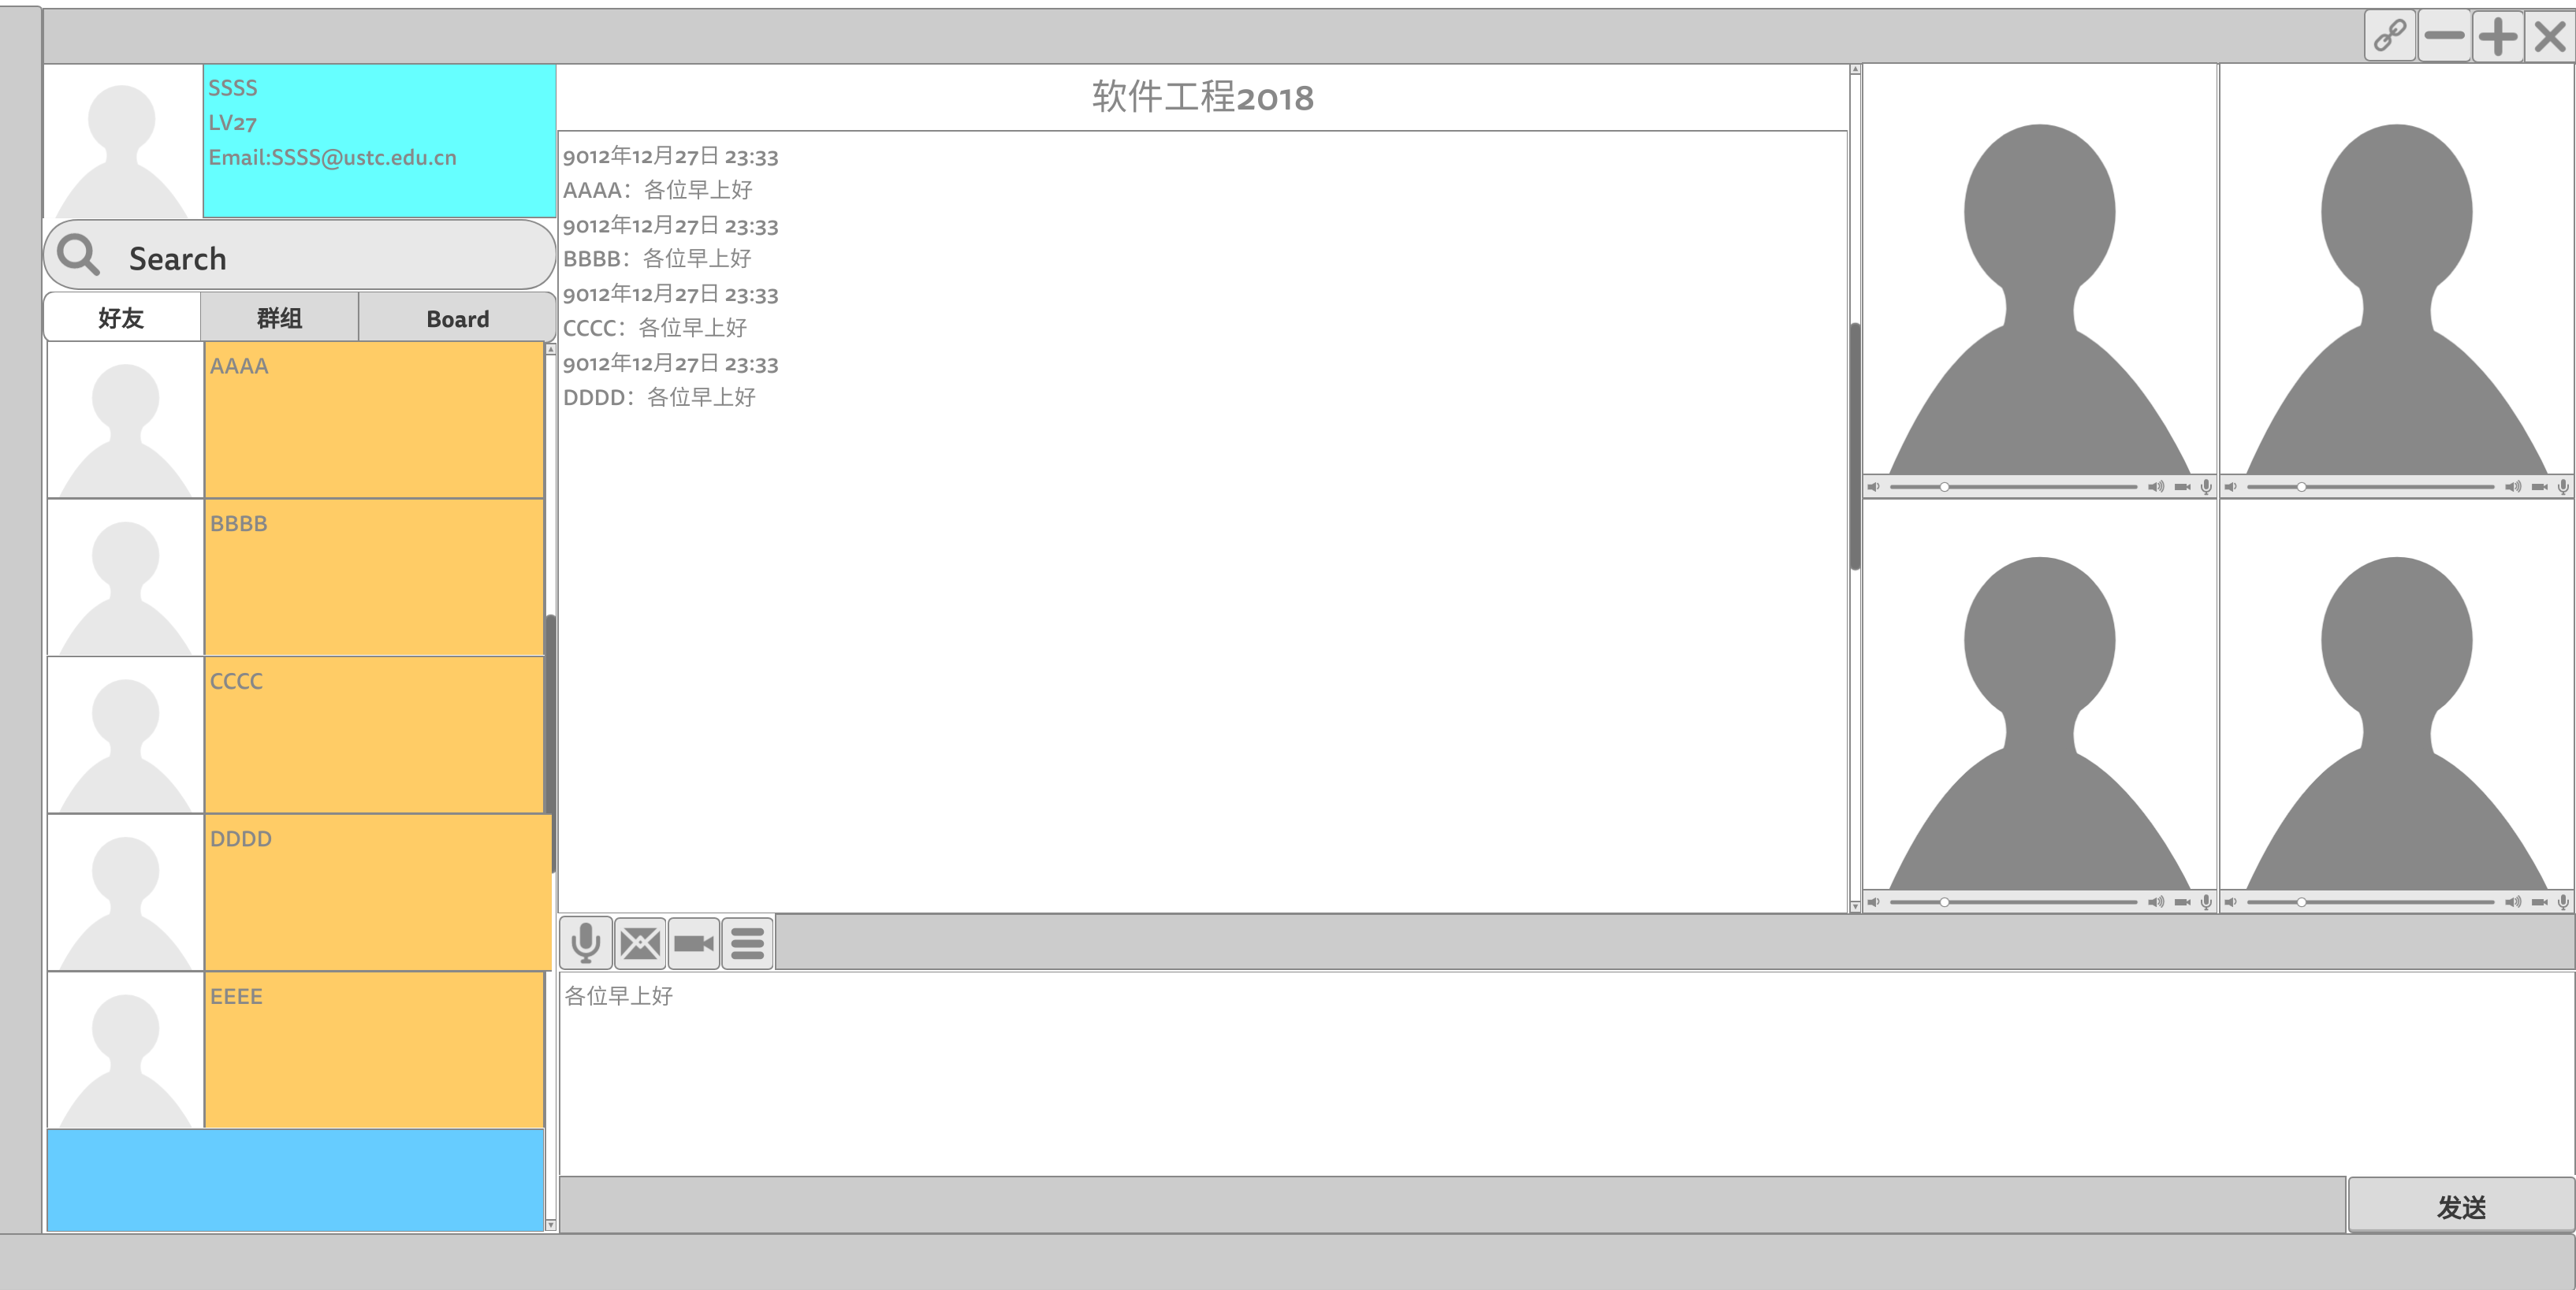
\includegraphics[scale = 0.175]{userinterface.png}\label{tab:classification}
	\caption{用户接口(PC端用户窗口)}\label{fig:noted-figure}
\end{figure}
\end{landscape}
\newpage
\subsection{软件接口}
\subsubsection{移动端}
	\begin{enumerate}
		\item 操作系统平台:Android 4.0以上,IOS 6以上
		\item 开发语言:JAVA
		\item 开发工具:Eclipse IDE 2019‑03
	\end{enumerate}
\subsubsection{PC端}
	\begin{enumerate}
		\item 操作系统平台:Windows7以上,Linux4.1.0以上,IOS 6以上
		\item 开发语言:JAVA
		\item 开发工具:Eclipse IDE 2019‑03
	\end{enumerate}
\subsubsection{服务器端}
	借助第三方服务器
%====================================================================================================================
% 详细描述与其他系统 /模块 /项目之间的接口
% 在此应描述如何使用其它(必需的)软件产品(例如,数据管理系统,操作系统,或算法工具包),
% 以及与其它应用系统的接口(例如,协议处理系统和数据库管理系统之间的接口)。
% 对每个必需的软件产品,应提供下列信息:
%	A. 名字、B. 助记符、C. 版本号、 D. 来源
% 对每个接口,本部分应:
%	A .	讨论与本软件产品相关的接口软件的目的。
%	B.	按消息/函数内容和格式定义接口。如果接口已在其它文档中很清楚地描述,就没有必要在这儿进行详细描述,但需说明应参考的文档。
%====================================================================================================================
\subsection{硬件接口}
\subsubsection{移动端}
	\begin{enumerate}
		\item 处理器要求:MSM800系列,Exynos5433以上,HelioX10以上,麒麟系列,A8以上
		% \item 运行环境:Android 4.0以上,IOS 6以上
		\item 内存要求:512MB以上
	\end{enumerate}
\subsubsection{PC端}
	\begin{enumerate}
		\item 处理器要求:Intel® Core™ i5以上
		% \item 运行环境:jdk11.0
		\item 内存要求:512MB以上
	\end{enumerate}
%====================================================================================================================
% 详细描述与硬件的接口
% 在此描述软件产品和系统硬件组件之间接口的逻辑特征,也包括支持哪些设备、怎样支持这些设备和协议等。
% 按软/硬件协议内容和格式定义接口。如果接口已在其它文档中很清楚地描述,就没有必要在这儿进行详细描述,但需说明应参考的文档。
%====================================================================================================================
\subsection{通讯接口}
使用TCP协议进行通讯,参考RFC793(https://tools.ietf.org/html/rfc793)。
%====================================================================================================================
% 详细描述通讯接口,如本地网络协议等。
% 按消息/函数内容和格式定义接口。如果接口已在其它文档中很清楚地描述,就没有必要在这儿进行详细描述,但需说明应参考的文档。
%====================================================================================================================
